\newpage
\section{Spannungsreferenzen}

\begin{multicols}{2}
	\subsection{Spannungsteiler}
	\begin{minipage}{0.4\linewidth}
		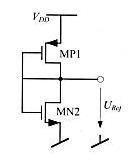
\includegraphics[width=2.5cm]{images/FET_Spannungsteiler.png} \\
	\end{minipage}
	\begin{minipage}{0.6\linewidth}
		Temperatur: S klein \\
		VDD / VSS: S = 1 \\
		Prozessvariation: S klein \\
	\end{minipage}
	
	\subsection{MOS-Diode}
	\begin{minipage}{0.4\linewidth}
		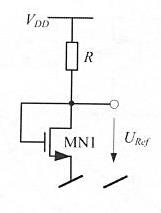
\includegraphics[width=3cm]{images/Diode_Spannungsteiler.png} \\
	\end{minipage}
	\begin{minipage}{0.6\linewidth}
		Temperatur: S klein \\
		VDD / VSS: S $<$ 1 \\
		Prozessvariation: S mittel \\
	\end{minipage}	

\subsection{Bandgap-Spannungsreferenz}
	\textbf{Grundprinzip:} \\
	\begin{minipage}{0.4\linewidth}
		\adjustbox{scale=0.5}{\begin{circuitikz}[scale=1.5]

\draw
	(0,0) node [ground] {}
	to [V<=$\Phi_t$] (0,1)
	to (1,1)
	(1,1.5) rectangle (2,0.5)
	(1.5,1) node {K}
	(2,1) to (3,1) to (3,1.5)
	(0,2) node [ground] {}
	to [V<=$V_D$] (0,3)
	to (3,3) to (3,2.5)
	(3,2) node {$+$} circle (0.5)
	(3.5,2) to [short] (4,2)
;

\end{circuitikz}} \\
	\end{minipage}
	\begin{minipage}{0.6\linewidth}
		$\Phi_t = \frac{kT}{e}$ \\($25.9mV$ bei Raumtemperatur) \\
		
		k: Boltzmann: $1.38\cdot 10^{-23}\frac{J}{K}$ \\
		T: Absolute Temperatur $[K]$ \\
		e: Elementarladung: $1.60\cdot 10^{-19}C$ \\
	\end{minipage}	

	\begin{minipage}{0.4\linewidth}
		\adjustbox{scale=0.5}{\begin{circuitikz}[scale=1.5, european]

\draw
	(0,0) node [ground] {}
	(1,0) node [ground] {}
	(2,0) node [ground] {}
	(3,0) node [ground] {}
	(4,0) node [ground] {}
	
	(0,1) node [pnp, xscale=-1] (T1) {}
	(3,1) node [pnp] (T2) {}

	(T1.B) -| (1,0)
	(T1.C) -- (0,0)
	(T1.E) -- (0,3)
	
	(T2.B) -| (2,0)
	(T2.C) -- (3,0)
	(T2.E) to [R=$R_3$] (3,3)
	
	(1.5,4) node [op amp, rotate=90, yscale=-1] (opamp) {}
	
	(0,3) -| (opamp.+)
	(3,3) -| (opamp.-)
	
	(0,3) to [R=$R_1$, *-] (0,5) to [short, -o] (4,5)
	(3,3) to [R=$R_2$, *-*] (3,5)
	
	(opamp.out) to [short, -*] (1.5,5)
	
	(4,4.5) to (4,0.5)
	(4,2.5) node [anchor=east] {$V_{ref}$}
		
	(0.5,1.5) -- (2.5,1.5)
	
	(1.5,1.5) node [anchor=south] {$\Delta V_D$}
;

\end{circuitikz}} \\
	\end{minipage}
	\begin{minipage}{0.6\linewidth}
		$V_{ref}=V_D+K\cdot \Phi_t$\\
		
		\textbf{Realisierung:}\\
		Die beiden Emitterflächen werden mit $A_1$ bzw. $A_2$ bezeichnet.\\
		$V_{ref}=V_{EB1}+\Phi_t\cdot\frac{R_2}{R_3}\cdot\ln\left(\frac{R_2}{R_1}\cdot\frac{A_2}{A_1}\right)$ \\
	\end{minipage}		

	

	
\end{multicols}



